\section{RNN}
\subsection{RNN前向传播}
简单起见,我们考虑一个无偏差项的循环神经网络,且激活函数为恒等映射($\phi(x)=x$)。设时间步 $t$ 的输入为单样本 $\boldsymbol{x}_t \in \mathbb{R}^d$,标签为 $y_t$,那么隐藏状态 $\boldsymbol{h}_t \in \mathbb{R}^h$的计算表达式为

$$
\boldsymbol{h}_t = \boldsymbol{W}_{hx} \boldsymbol{x}_t + \boldsymbol{W}_{hh} \boldsymbol{h}_{t-1},
$$

其中$\boldsymbol{W}_{hx} \in \mathbb{R}^{h \times d}$和$\boldsymbol{W}_{hh} \in \mathbb{R}^{h \times h}$是隐藏层权重参数。设输出层权重参数$\boldsymbol{W}_{qh} \in \mathbb{R}^{q \times h}$,时间步$t$的输出层变量$\boldsymbol{o}_t \in \mathbb{R}^q$计算为

$$
\boldsymbol{o}_t = \boldsymbol{W}_{qh} \boldsymbol{h}_{t}.
$$

设时间步$t$的损失为$\ell(\boldsymbol{o}_t, y_t)$。时间步数为$T$的损失函数$L$定义为

$$
L = \frac{1}{T} \sum_{t=1}^T \ell (\boldsymbol{o}_t, y_t).
$$

我们将$L$称为有关给定时间步的数据样本的目标函数。
\begin{figure}[h]
	\centering
	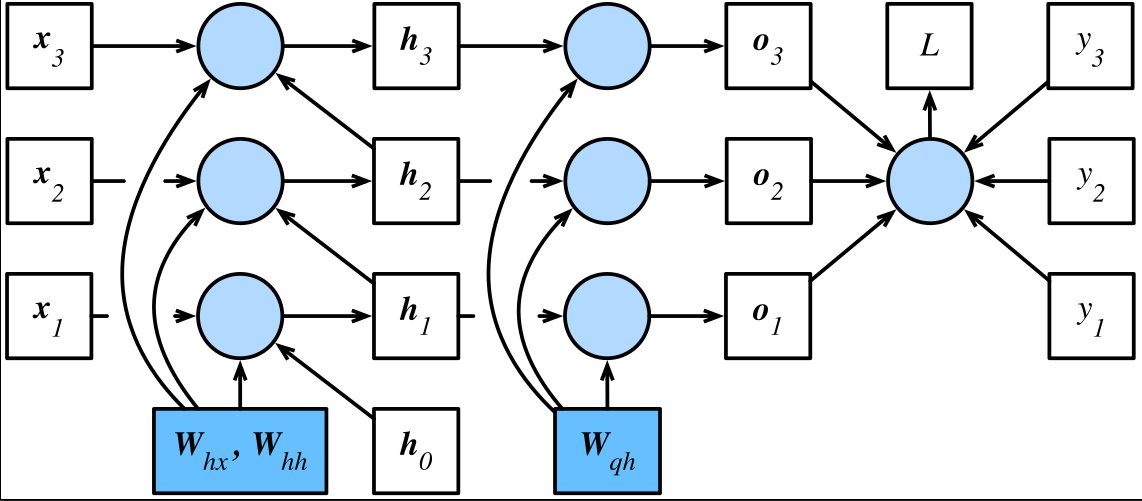
\includegraphics[width=\textwidth]{./img/code/RNN/ttbp.png}
\end{figure}

\subsection{通过时间反向传播}

模型的参数是 $\boldsymbol{W}_{hx}$, $\boldsymbol{W}_{hh}$ 和 $\boldsymbol{W}_{qh}$。链式法则的运算符用prod表示。
\begin{enumerate}
	\item $\partial L/\partial \boldsymbol{W}_{qh}$
	\begin{equation}
		\frac{\partial L}{\partial \boldsymbol{W}_{qh}} 
		= \sum_{t=1}^T \text{prod}\left(\frac{\partial L}{\partial \boldsymbol{o}_t}, \frac{\partial \boldsymbol{o}_t}{\partial \boldsymbol{W}_{qh}}\right) 
		= \sum_{t=1}^T \frac{\partial L}{\partial \boldsymbol{o}_t} \boldsymbol{h}_t^\top.
	\end{equation}
	\item $\partial L/\partial \boldsymbol{W}_{hx}$
	\begin{equation}
		\frac{\partial L}{\partial \boldsymbol{W}_{hx}} 
		= \sum_{t=1}^T \text{prod}\left(\frac{\partial L}{\partial \boldsymbol{h}_t}, \frac{\partial \boldsymbol{h}_t}{\partial \boldsymbol{W}_{hx}}\right) 
		= \sum_{t=1}^T \frac{\partial L}{\partial \boldsymbol{h}_t} \boldsymbol{x}_t^\top
	\end{equation}
	\item $\partial L/\partial \boldsymbol{W}_{hh}$
	\begin{equation}
		\frac{\partial L}{\partial \boldsymbol{W}_{hh}} 
		= \sum_{t=1}^T \text{prod}\left(\frac{\partial L}{\partial \boldsymbol{h}_t}, \frac{\partial \boldsymbol{h}_t}{\partial \boldsymbol{W}_{hh}}\right) 
		= \sum_{t=1}^T \frac{\partial L}{\partial \boldsymbol{h}_t} \boldsymbol{h}_{t-1}^\top.
	\end{equation}
\end{enumerate}
其中,目标函数有关各时间步输出层变量的梯度$\partial L/\partial \boldsymbol{o}_t \in \mathbb{R}^q$很容易计算:
\begin{equation}
	\frac{\partial L}{\partial \boldsymbol{o}_t} =  \frac{\partial \ell (\boldsymbol{o}_t, y_t)}{T \cdot \partial \boldsymbol{o}_t}.	
\end{equation}
目标函数有关时间步隐藏状态的梯度$\partial L/\partial \boldsymbol{h}_t \in \mathbb{R}^h$。依据链式法则,我们得到
\begin{equation}
	\frac{\partial L}{\partial \boldsymbol{h}_t} 
	= \sum_{i=t}^T {\left(\boldsymbol{W}_{hh}^\top\right)}^{T-i} \boldsymbol{W}_{qh}^\top \frac{\partial L}{\partial \boldsymbol{o}_{T+t-i}}.
\end{equation}
由上式中的指数项可见,当时间步数 $T$ 较大或者时间步 $t$ 较小时,目标函数有关隐藏状态的梯度较容易出现衰减和爆炸。这也会影响其他包含$\partial L / \partial \boldsymbol{h}_t$项的梯度。

